\documentclass{article}
\usepackage{graphicx}

\title{
\textbf{pacman-racket} \\
\textit{Develeper Guide}\\
A pragmatic implementation of Pacman in Racket
}

\author{
    Alessandro Zanzi,
    Filippo Piloni,\\
    Jeferson Morales Mariciano,
    Paolo Deidda
}
\date{
USI \\
Faculty of Informatics \\
[\baselineskip]  2021/2022
}


\begin{document}
%%%%%%%%%%%%%%%%%%%%%%%
%%%%%%%%%%%%%%%%%%%%%%%
%%%%%%%%%%%%%%%%%%%%%%%
\begin{titlepage}
\maketitle  

\end{titlepage}
 %%%%%%%%%%%%%%%%%%%%%%%
 %%%%%%%%%%%%%%%%%%%%%%%
 %%%%%%%%%%%%%%%%%%%%%%%
 \begin{abstract}
Conceptualization, research and thinking out-of-the-box
to implement the well-known classic game Pac-man
using the Racket functional programming language.\\
To develop this project, our group used abstractions and open-source tools to develop five files using Racket and linking them together to clarify the divisions between the various parts of the program and their respective functions.\\
To better organize with this project, we used several instruments such as GitHub to be able to work at the program at any momen t remaining updated.\\
Using the knowledge developed during the lectures and the guides provided by Racket Documentation, the result of the project was a working revisited version of the game Pac-Man composed by one level where the ghosts move using a contrast logic that considers Pac-Man position in the map.

 \end{abstract}
\clearpage
%%%%%%%%%%%%%%%%%%%%%%%
%%%%%%%%%%%%%%%%%%%%%%%
%%%%%%%%%%%%%%%%%%%%%%%
 \tableofcontents
 \clearpage
 %%%%%%%%%%%%%%%%%%%%%%%
 %%%%%%%%%%%%%%%%%%%%%%%
 %%%%%%%%%%%%%%%%%%%%%%%
 \section{Analysis}
 
 \hspace{0.5cm}\textbf{Modularity}\\
 In order for the group to work in parallel on the project we created several files on which each of us worked simultaneously. These files were then interconnected with the built in function of Racket "require" followed by the name of the file.

   \begin{center}
 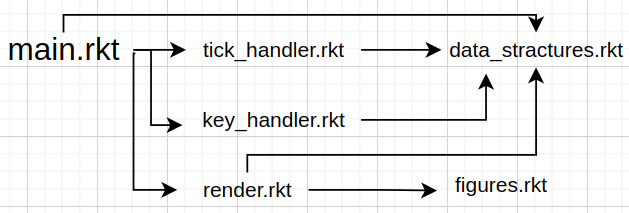
\includegraphics[width=12cm]{images/dependency_tree.png}
 \end{center}
 
 \textbf{Bottom-up approach}\\
 We developed the code decomposing the functions needed in the simplest possible problems, we then conveyed them in higher grade functions. This allowed a design recepie with more tests making the debugging process easier.
 
  \begin{center}
 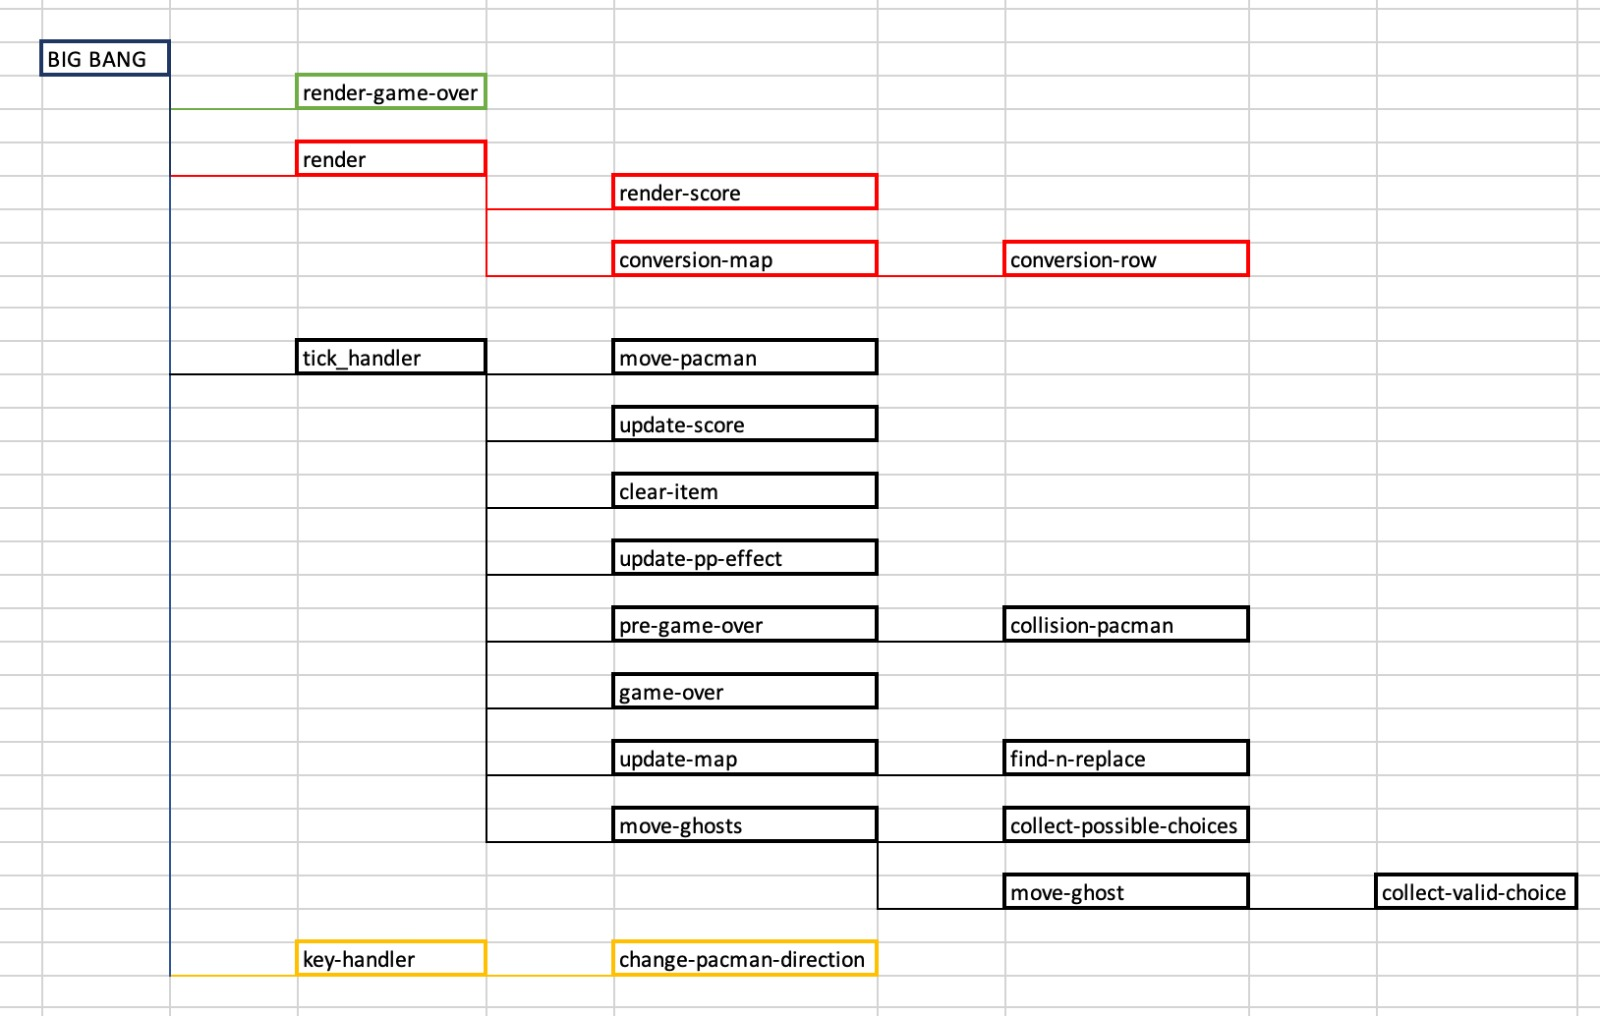
\includegraphics[width=12cm]{images/dependency_tree2.jpeg}
 \end{center}
 
 %%%%%%%%%%%%%%%%%%%%%%%
 %%%%%%%%%%%%%%%%%%%%%%%
 %%%%%%%%%%%%%%%%%%%%%%%
 \section{Sofware design}
 \subsection{Tools}
 \hspace{0.5cm}\LaTeX \\
 Used for the user guide\\
 
 \textit{Flowchart}\\
 Used to create the dependency trees so each member of the group had a clear view of the whole project.
 

 \subsection{UI}
\begin{center}
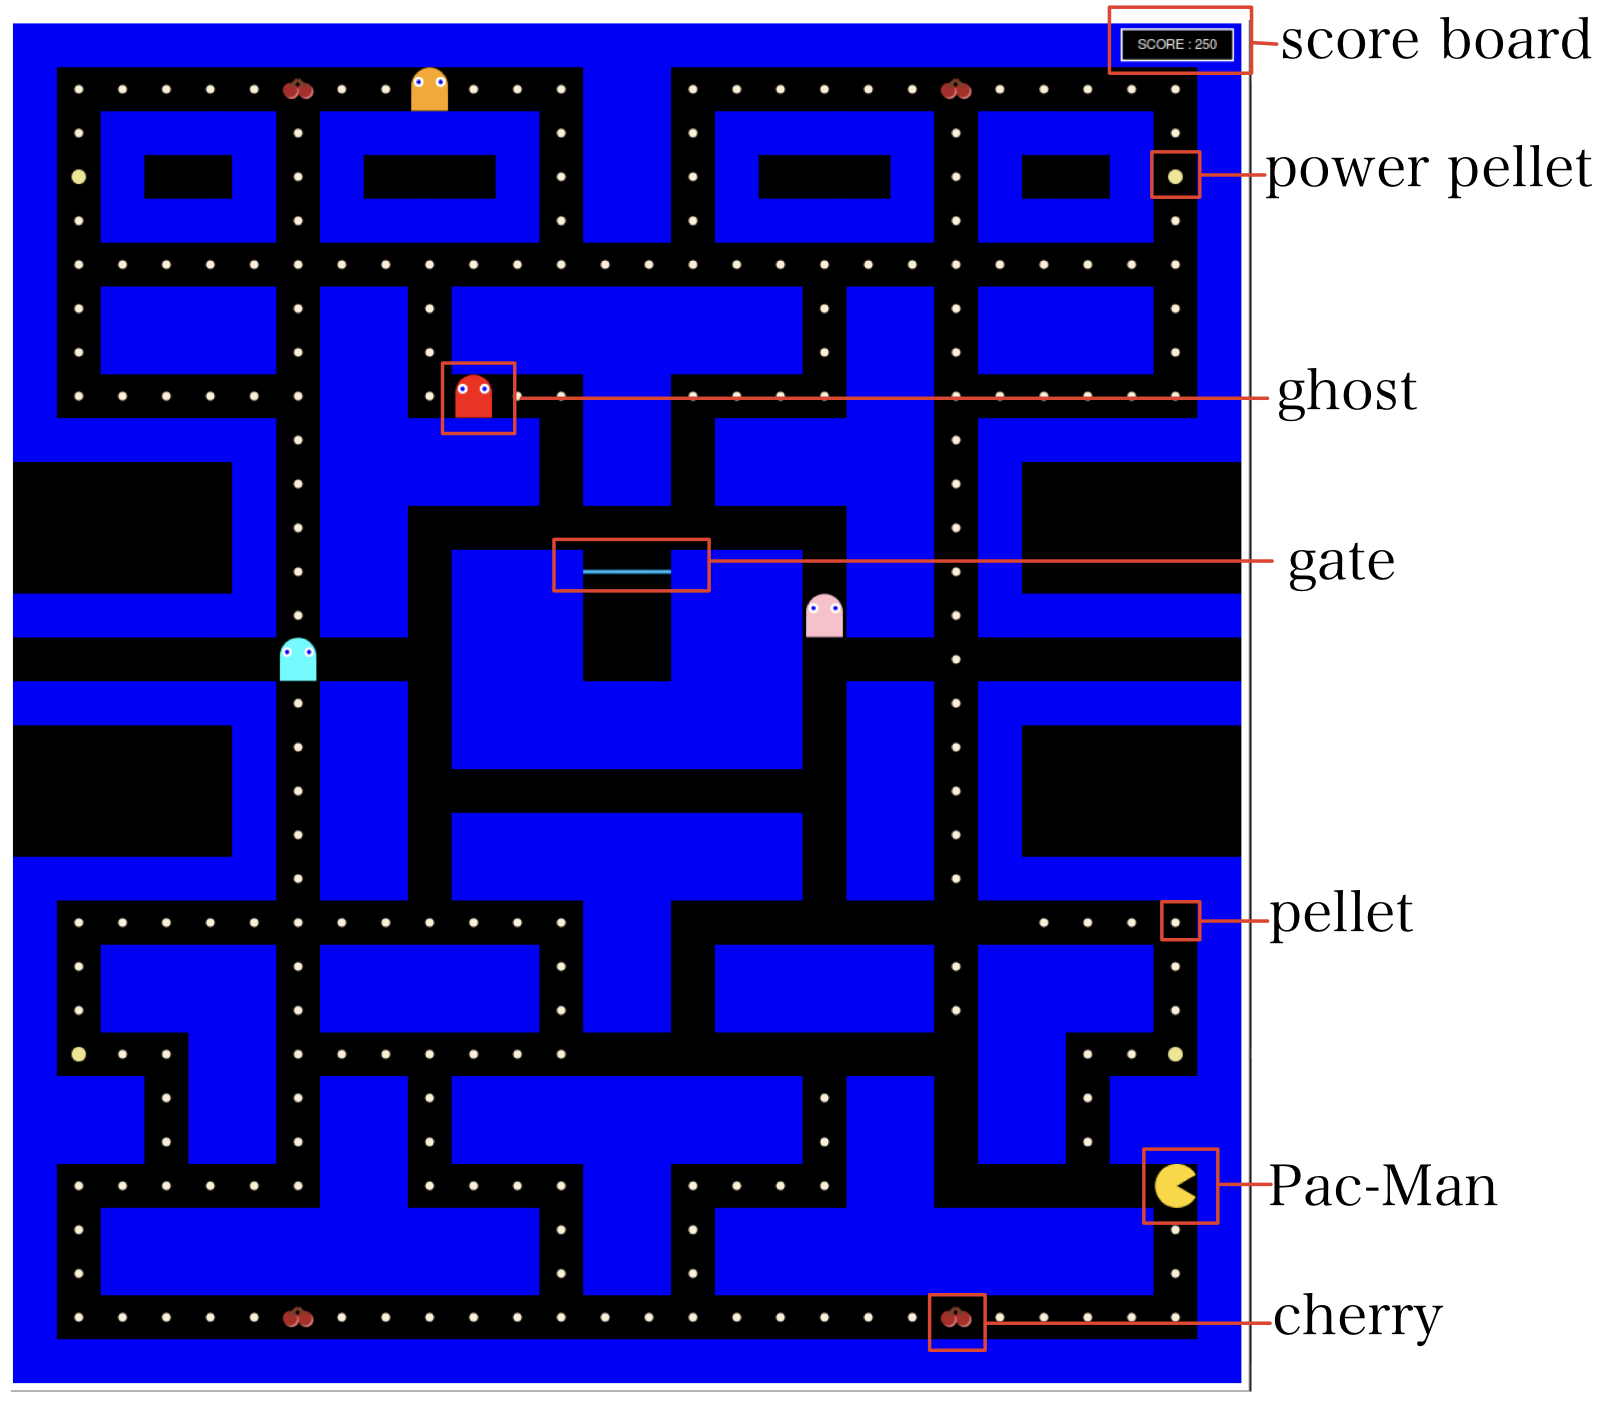
\includegraphics[width=12cm]{./images/user_interface.png}
\end{center}
The gaming window is completely occupied by the game screen (figure above), which is composed by the main area and the score display. While the score display keep track of the actual score, the main area is the most important part of the game. It is composed by several images that rapresents the part of the game, such as the ghosts, pac-man, the pellets and the powerpellets.

%%%%%%%%%%%%%%%%%%%%%%%
%%%%%%%%%%%%%%%%%%%%%%%
%%%%%%%%%%%%%%%%%%%%%%%
 \section{Software Development}

 \subsection{Source Code}
 The project is developed on the idea of creating a map of squares placed side by side that make up the game world. To run the game we work on a "logic map" which is composed by strings of characters, that form lines, one above the other. This set of lines create a vector that will be the game logic map. All the engine functions that we have developed in the source code operate on the lines of this vector in a recursive manner modifying and moving the various characters.To give life to the game we then have created a render function that takes each character of the logic map and associates the corresponding image.\\
 
 \begin{center}
 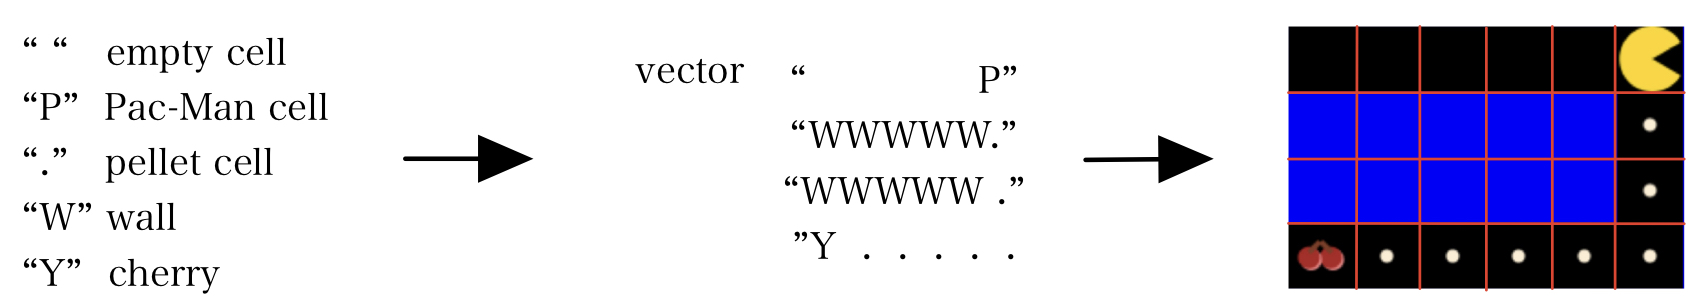
\includegraphics[width=12cm]{./images/vector.jpeg}
 \end{center}

 Characters such as Pac-Man and ghosts are defined by structures in the code. Pac-Man direction movement is defined by the key-events (up, down, left, right) while instead the movement of ghosts is defined randomly until Pac-Man is in one of the near cells, because when this happens they start to follow him.
 As an example for Pacman, the validity of its moves is verified by checking what is in the current and next cell and the event that is about to happen like collision with a ghost, a wall , a powerpellet, etc. Likewise, at runtime when there is a wall in the next box, the move-pacman function returns pacman to the same position, if instead there is a ghost the game over event will be triggered.
 
 \subsection{Tools}
 
 \hspace{0.5cm}\textit{Racket}\\
 Programming language used to develop the game.\\
 

 \textit{drRacket}\\
 As Integrated development environment (IDE).\\
 
 \textit{VCS Git}\\
Software that we used to track changes in the project set of files, in order to each of us to develop source code and share it in an easy and reliable way: low risk of data loss and archives with the previus versions ready to back up if needed.\\

 \textit{Hosting GiHub}\\
The whole project is physically stored in a private repository located on GitHub's servers. This granted us to access the work at any time in any place as long as we had internet connection.

\subsection{Libraries}
 \hspace{0.5cm}\textit{Universe}\\
 Teachpack that implements and provides the functionality for creating interactive, graphical programs that consist of plain mathematical functions.
 
 \textit{Image}\\
The image teachpack provides a number of basic image construction functions, along with combinators for building more complex images out of existing images.

%%%%%%%%%%%%%%%%%%%%%%%
%%%%%%%%%%%%%%%%%%%%%%%
%%%%%%%%%%%%%%%%%%%%%%%

\end{document}
